\documentclass[12pt]{article}
\usepackage[utf8]{inputenc}
\usepackage[brazil]{babel}
\usepackage{setspace}
\usepackage{float}
\usepackage[pdftex]{graphicx}
\usepackage{float}
\usepackage{url}

\setlength{\paperheight}{29.7cm}
\setlength{\footskip}{1.0cm}
\setlength{\textheight}{21.0cm}
\setlength{\textwidth}{17.0cm}
\setlength{\oddsidemargin}{0.0cm}
\setlength{\topmargin}{0.0cm} 

\newsavebox{\fmbox}
\newenvironment{fmpage}[1][.8\textwidth]{
    \begin{lrbox}{\fmbox}
      \begin{minipage}{#1}
        \small
}{
      \end{minipage}
    \end{lrbox}\fbox{\usebox{\fmbox}}
}

\newenvironment{exemplo}{
  \begin{center}
    \begin{fmpage}\small
      \textbf{Exemplo:}\\
}{
    \end{fmpage}
  \end{center}
}

\newenvironment{exemploc}{
  \begin{center}
    \begin{fmpage}\small
      \emph{continuação...}\\
}{
    \end{fmpage}
  \end{center}
}

\title{Relatório MAC0209 - IME - USP}

\author{Davi de Menezes Pereira, 11221988\\
Gustavo de Medeiros Carlos, 11276298\\
Lucas Irineu Rebouças Guimarães, 11221713\\
Luciano Rodrigues Saraiva Leão, 11221817\\
Luiza Barros Reis Soezima, 11221842\\
Marcos Siolin Martins, 11221709}

\begin{document}

\maketitle

\begin{abstract}
    Este trabalho tem o intuito de utilizar a modelagem de alguns tipos de movimentos, descritas nos livros do professor Herch Moysés Nussenzveig, bem como simulá-los utilizando as soluções analítica e de Euler da equação diferencial que descreve sua modelagem.    
\end{abstract}

\tableofcontents

\newpage

\section{Introdução}

Os movimentos a serem simulados são:
\begin{itemize}
  \item Queda Livre;
  \item Descida na Rampa;
  \item Pêndulo;
  \item Movimento Retilíneo Uniforme e Uniformemente Acelerado;
  \item Movimento Circular;
\end{itemize}

\subsection{Motivação}

Este projeto tem o intuito de simular os movimentos modelados agregando um maior conhecimento de como esse modelos podem ser usados com o uso do computador. O projeto também exercita a organização quando se trabalha em um projeto em equipe, bem como as etapas necessárias para a conclusão do projeto de maneira apropriada.

\subsection{Objetivos}

Dentre os objetivos deste experimento, estão:
\begin{itemize}
  \item Implementar e simular cada um dos modelos dos movimentos utilizando as modelagens apresentadas no enunciado do exercício programa e no livro do professor Nussenzveig, através da resolução da equação diferencial apresentada (solução analítica) ou pela aproximação das derivadas por diferenças finitas (solução de Euler);
  \item Comparar as duas implementações para cada movimento, "plotando" os resultados obtidos;
  \item Fazer uma animação utilizando animação gráfica para mostrar como se comporta a trajetória do movimento;
\end{itemize}

\section{Materiais e métodos}

Nesta seção, descreva o cronograma de desenvolvimento realizado para o projeto (Ver Figura~\ref{fig:gantt}).

\begin{figure}[H]
  \begin{center}    
    \includegraphics[scale = 0.3]{ganttchart.png}
    \includegraphics[width=0.7\textwidth]{chart.png}
    \caption{\label{fig:gantt} Gantt chart adotado para o desenvolvimento do projeto.}
  \end{center}
\end{figure}

\section{Resultados Experimentais}

\subsection{Movimento Retilíneo Uniforme e Uniformemente Variado}
\begin{figure}[H]
  \centering
  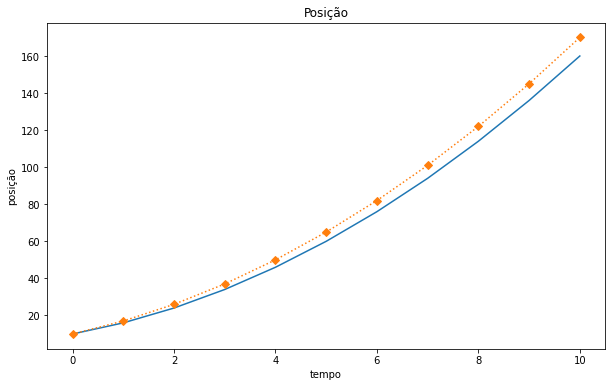
\includegraphics[scale = 0.6]{imagens/dt=1 tf=10 posicao.png}
  \caption{Aceleração = 2, velocidade inicial = 5, posição inicial = 10, dt = 1}
\end{figure}
\begin{figure}[H]
  \centering
  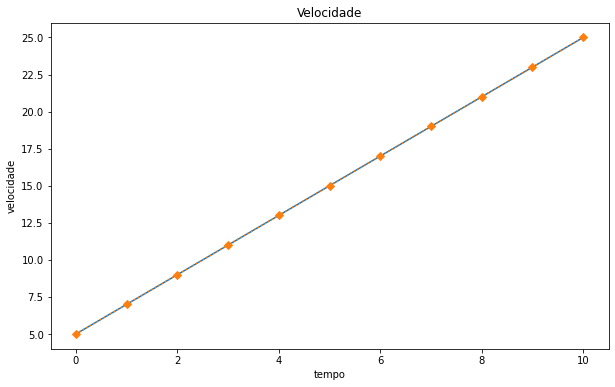
\includegraphics[scale = 0.6]{imagens/dt=1 tf=10 velocidade.png}
  \caption{Aceleração = 2, velocidade inicial = 5, posição inicial = 10, dt = 1}
\end{figure}
\begin{figure}[H]
  \centering
  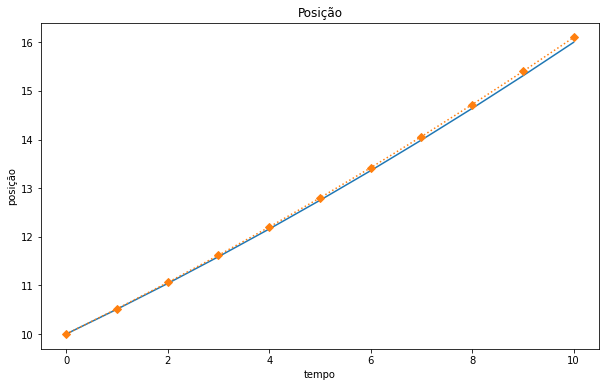
\includegraphics[scale = 0.6]{imagens/dt=0.1 tf=1 posicao.png}
  \caption{Aceleração = 2, velocidade inicial = 5, posição inicial = 10, dt = 0.1}
\end{figure}
\begin{figure}[H]
  \centering
  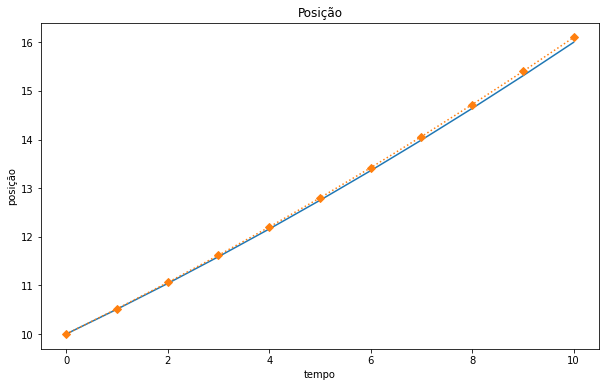
\includegraphics[scale = 0.6]{imagens/dt=0.1 tf=1 posicao.png}
  \caption{Aceleração = 2, velocidade inicial = 5, posição inicial = 10, dt = 0.1}
\end{figure}
\subsection{Queda Livre}
\begin{figure}[H]
  \centering
  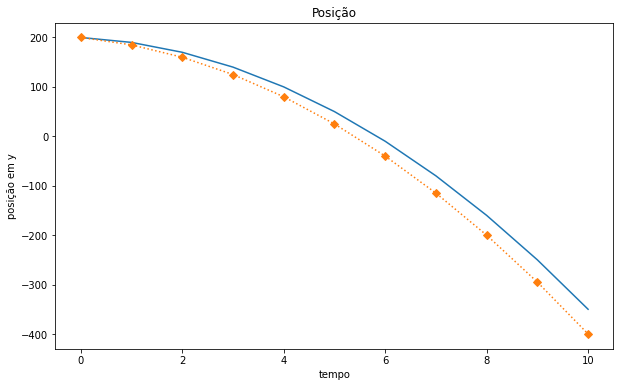
\includegraphics[scale = 0.6]{imagens/dt=1 tf=10 posicao em y.png}
  \caption{Aceleração = 10, velocidade inicial = -5, posição inicial = 200, dt = 1}
\end{figure}
\begin{figure}[H]
  \centering
  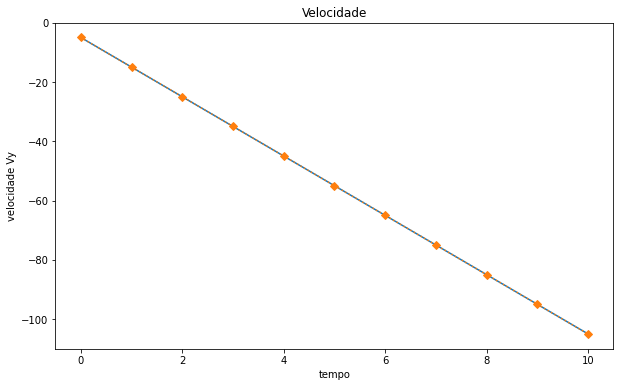
\includegraphics[scale = 0.6]{imagens/dt=1 tf=10 velocidade em y.png}
  \caption{Aceleração = 10, velocidade inicial = -5, posição inicial = 200, dt = 1}
\end{figure}
\begin{figure}[H]
  \centering
  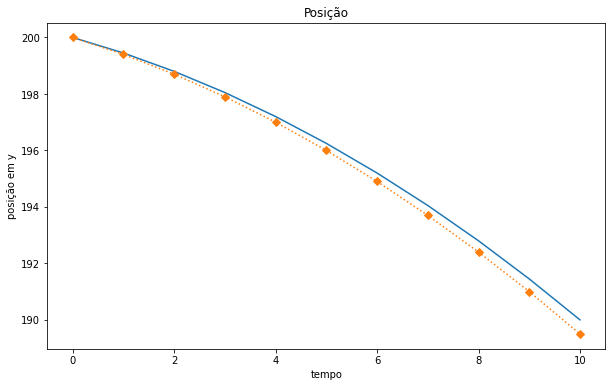
\includegraphics[scale = 0.6]{imagens/dt=0.1 tf=1 posicao em y.png}
  \caption{Aceleração = 10, velocidade inicial = -5, posição inicial = 200, dt = 0.1}
\end{figure}
\begin{figure}[H]
  \centering
  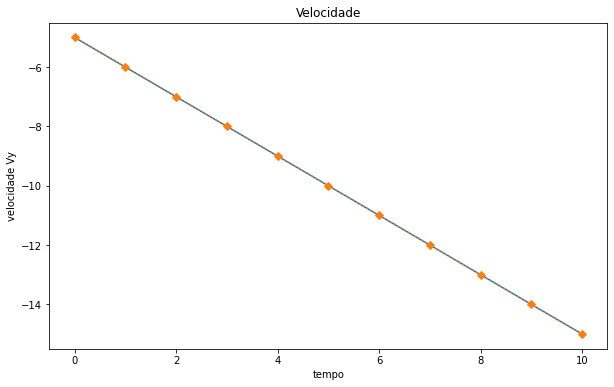
\includegraphics[scale = 0.6]{imagens/dt=0.1 tf=1 velocidade em y.png}
  \caption{Aceleração = 10, velocidade inicial = -5, posição inicial = 200, dt = 0.1}
\end{figure}
\begin{figure}[H]
  \centering
  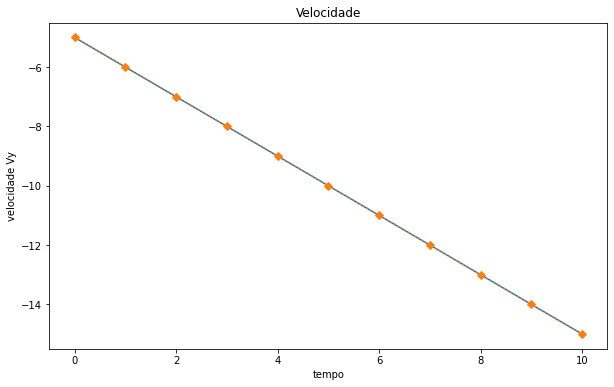
\includegraphics[scale = 0.6]{imagens/dt=0.1 tf=1 velocidade em y.png}
  \caption{Aceleração = 10, velocidade inicial = -5, posição inicial = 200, dt = 0.1}
\end{figure}
\subsection{Pêndulo}
\begin{figure}[H]
  \centering
  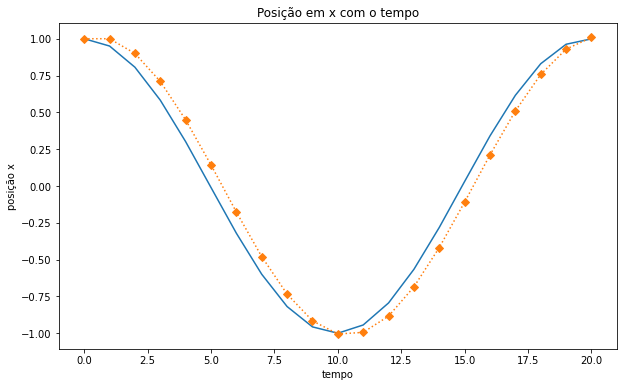
\includegraphics[scale = 0.6]{imagens/(pendulo)dt=1tf=20posicaox.png}
  \caption{$x_0$ = 1, $y_0$ = 0.005, velocidade inicial = -5, posição inicial = 1, A = 1, $\Phi_0$ = 0, $\theta_0 = 0$, g = 10, L = 100, dt = 1}
\end{figure}
\begin{figure}[H]
  \centering
  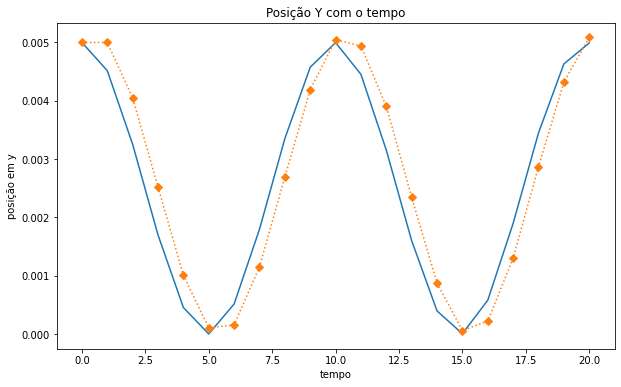
\includegraphics[scale = 0.6]{imagens/(pendulo)dt=1tf=20posicaoy.png}
  \caption{$x_0$ = 1, $y_0$ = 0.005, velocidade inicial = -5, posição inicial = 1, A = 1, $\Phi_0$ = 0, $\theta_0 = 0$, g = 10, L = 100, dt = 1}
\end{figure}
\begin{figure}[H]
  \centering
  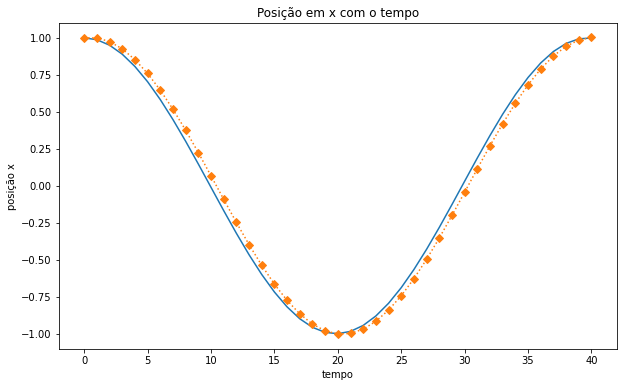
\includegraphics[scale = 0.6]{imagens/(pendulo)dt=0.5tf=20posicaox.png}
  \caption{$x_0$ = 1, $y_0$ = 0.005, velocidade inicial = -5, posição inicial = 1, A = 1, $\Phi_0$ = 0, $\theta_0 = 0$, g = 10, L = 100, dt = 0.5}
\end{figure}
\begin{figure}[H]
  \centering
  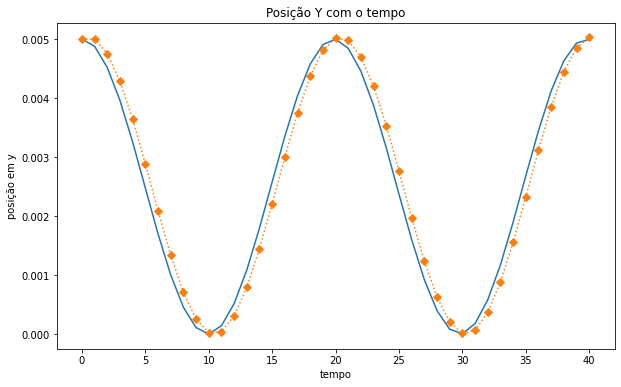
\includegraphics[scale = 0.6]{imagens/(pendulo)dt=0.5tf=20posicaoy.png}
  \caption{$x_0$ = 1, $y_0$ = 0.005, velocidade inicial = -5, posição inicial = 1, A = 1, $\Phi_0$ = 0, $\theta_0 = 0$, g = 10, L = 100, dt = 0.5}
\end{figure}
\subsection{Bloco em rampa}
\begin{figure}[H]
  \centering
  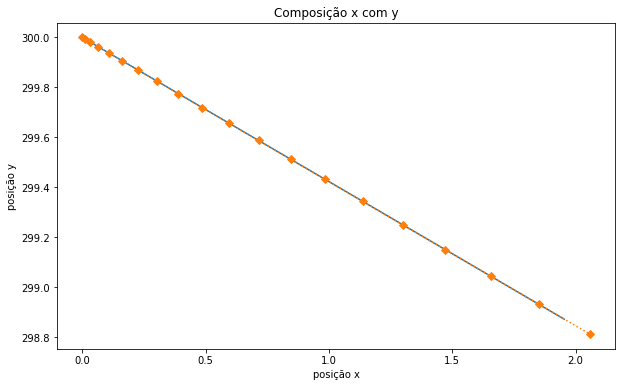
\includegraphics[scale = 0.6]{imagens/(blocoemrampa)composicaoxydt=0.05tf=1.png}
  \caption{$\theta = \frac{\pi}{6}$, $x_0 = 0$, $y_0 = 300$, $g = 10$, $v_0 = 100$, dt = 0.05}
\end{figure}
\begin{figure}[H]
  \centering
  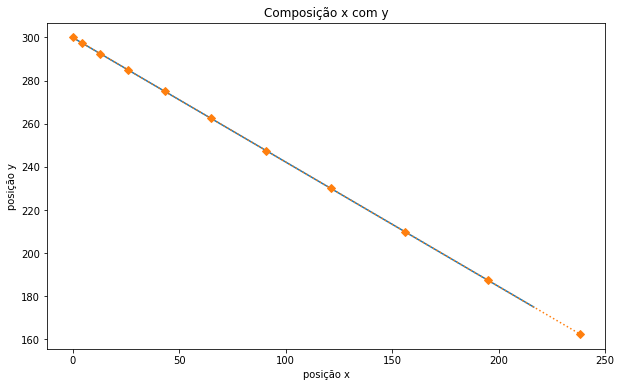
\includegraphics[scale = 0.6]{imagens/(blocoemrampa)composicaoxydt=1tf=10.png}
  \caption{$\theta = \frac{\pi}{6}$, $x_0 = 0$, $y_0 = 300$, $g = 10$, $v_0 = 100$, dt = 1}
\end{figure}
\begin{figure}[H]
  \centering
  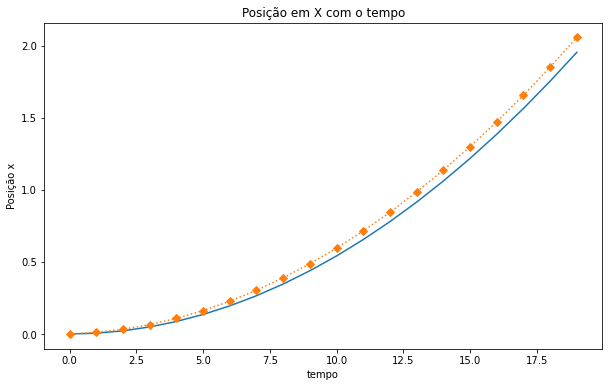
\includegraphics[scale = 0.6]{imagens/(blocoemrampa)posicaoxdt=0.05tf=1.png}
  \caption{$\theta = \frac{\pi}{6}$, $x_0 = 0$, $y_0 = 300$, $g = 10$, $v_0 = 100$, dt = 0.05}
\end{figure}
\begin{figure}[H]
  \centering
  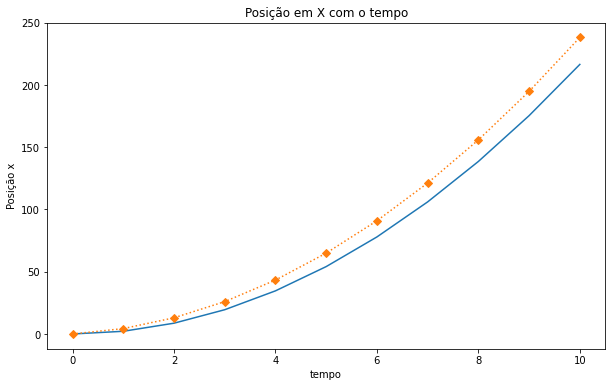
\includegraphics[scale = 0.6]{imagens/(blocoemrampa)posicaoxdt=1tf=10.png}
  \caption{$\theta = \frac{\pi}{6}$, $x_0 = 0$, $y_0 = 300$, $g = 10$, $v_0 = 100$, dt = 1}
\end{figure}
\begin{figure}[H]
  \centering
  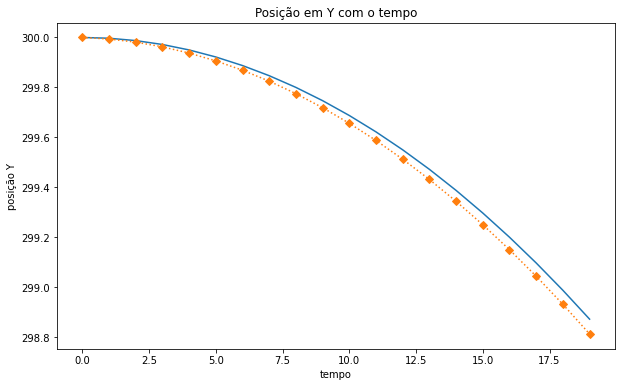
\includegraphics[scale = 0.6]{imagens/(blocoemrampa)posicaoydt=0.05tf=1.png}
  \caption{$\theta = \frac{\pi}{6}$, $x_0 = 0$, $y_0 = 300$, $g = 10$, $v_0 = 100$, dt = 0.05}
\end{figure}
\begin{figure}[H]
  \centering
  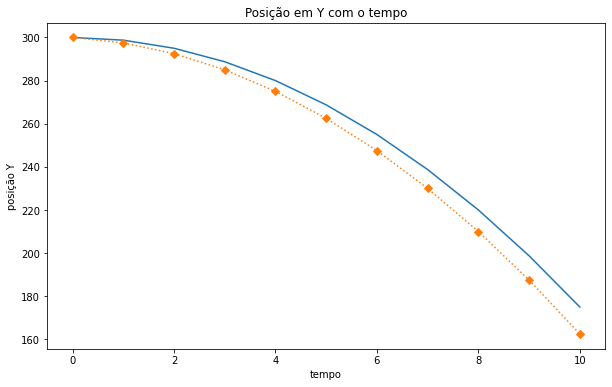
\includegraphics[scale = 0.6]{imagens/(blocoemrampa)posicaoydt=1tf=10.png}
  \caption{$\theta = \frac{\pi}{6}$, $x_0 = 0$, $y_0 = 300$, $g = 10$, $v_0 = 100$, dt = 1}
\end{figure}
\begin{figure}[H]
  \centering
  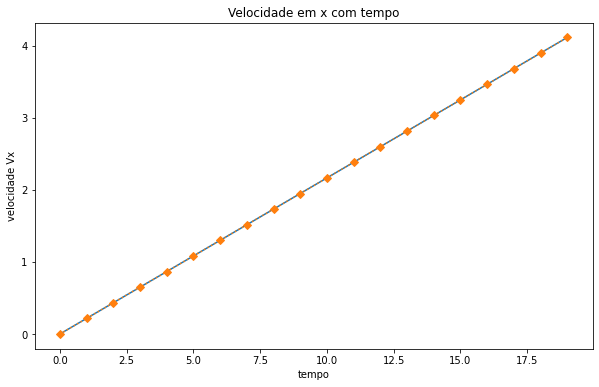
\includegraphics[scale = 0.6]{imagens/(blocoemrampa)velocidadexdt=0.05tf=1.png}
  \caption{$\theta = \frac{\pi}{6}$, $x_0 = 0$, $y_0 = 300$, $g = 10$, $v_0 = 100$, dt = 0.05}
\end{figure}
\begin{figure}[H]
  \centering
  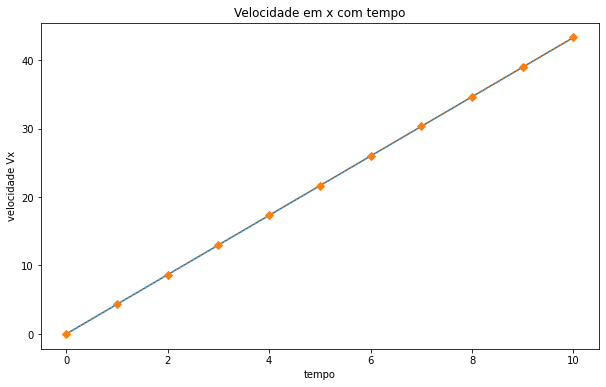
\includegraphics[scale = 0.6]{imagens/(blocoemrampa)velocidadexdt=1tf=10.png}
  \caption{$\theta = \frac{\pi}{6}$, $x_0 = 0$, $y_0 = 300$, $g = 10$, $v_0 = 100$, dt = 1}
\end{figure}
\begin{figure}[H]
  \centering
  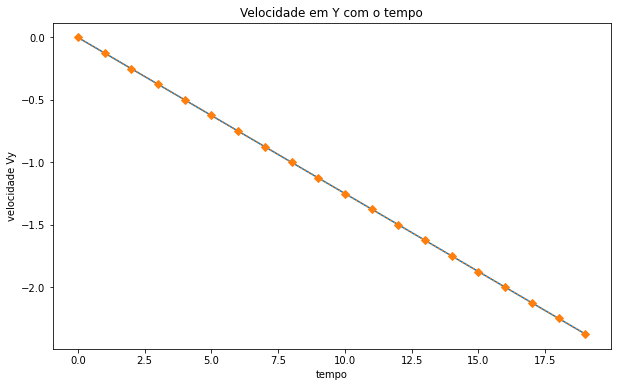
\includegraphics[scale = 0.6]{imagens/(blocoemrampa)velocidadeydt=0.05tf=1.png}
  \caption{$\theta = \frac{\pi}{6}$, $x_0 = 0$, $y_0 = 300$, $g = 10$, $v_0 = 100$, dt = 0.05}
\end{figure}
\begin{figure}[H]
  \centering
  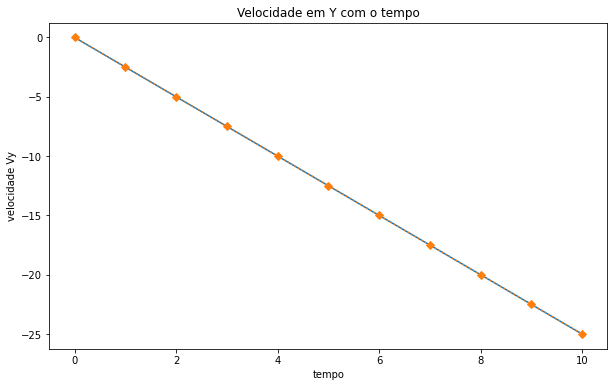
\includegraphics[scale = 0.6]{imagens/(blocoemrampa)velocidadeydt=1tf=10.png}
  \caption{$\theta = \frac{\pi}{6}$, $x_0 = 0$, $y_0 = 300$, $g = 10$, $v_0 = 100$, dt = 1}
\end{figure}
\subsection{Movimento Circular Uniforme}
\begin{figure}[H]
  \centering
  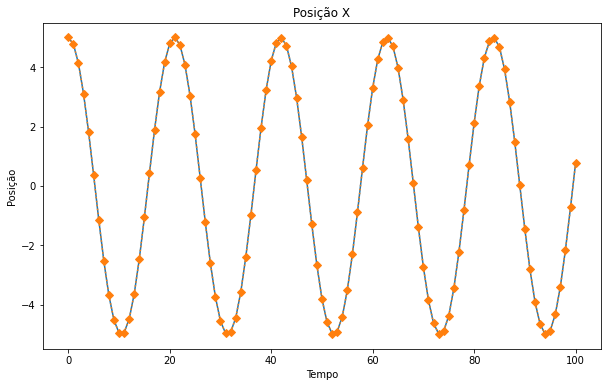
\includegraphics[scale = 0.6]{imagens/(mcu)posicaoxdt=0.05tf=5.png}
  \caption{$R = 5$, $x_0 = R = 5$, $y_0 = 0$, $\omega = 6$, dt = 0.05}
\end{figure}
\begin{figure}[H]
  \centering
  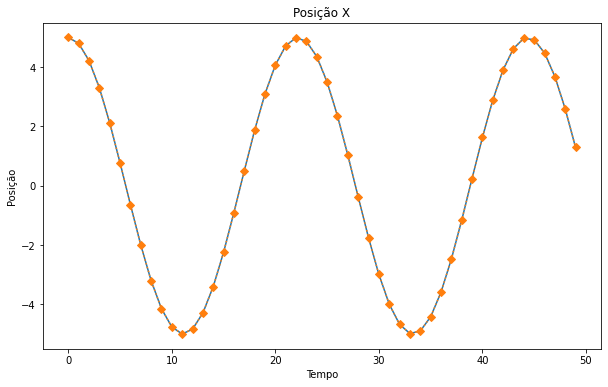
\includegraphics[scale = 0.6]{imagens/(mcu)posicaoxdt=1tf=50.png}
  \caption{$R = 5$, $x_0 = R = 5$, $y_0 = 0$, $\omega = 6$, dt = 1}
\end{figure}
\begin{figure}[H]
  \centering
  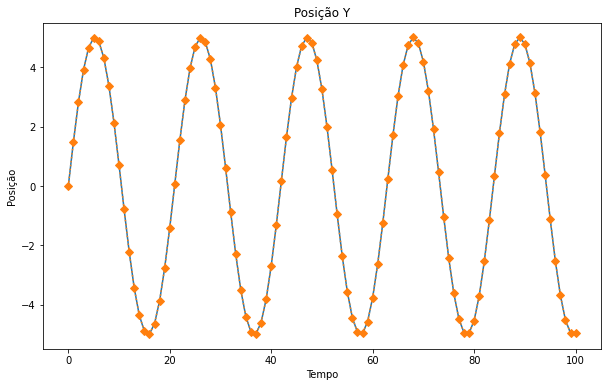
\includegraphics[scale = 0.6]{imagens/(mcu)posicaoydt=0.05tf=5.png}
  \caption{$R = 5$, $x_0 = R = 5$, $y_0 = 0$, $\omega = 6$, dt = 0.05}
\end{figure}
\begin{figure}[H]
  \centering
  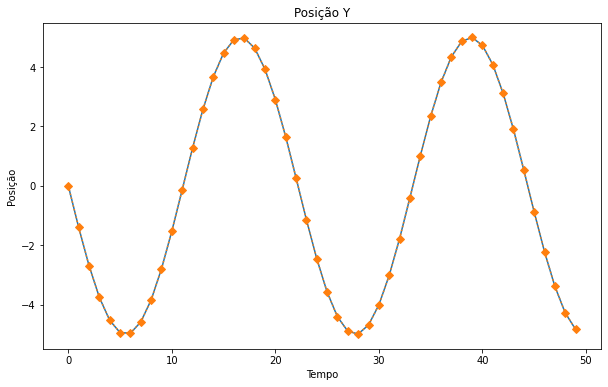
\includegraphics[scale = 0.6]{imagens/(mcu)posicaoydt=1tf=50.png}
  \caption{$R = 5$, $x_0 = R = 5$, $y_0 = 0$, $\omega = 6$, dt = 1}
\end{figure}
\section{Conclusão}

Através das simulações e dos resultados experimentais encontrados é possível concluir o quão melhor a solução analítica é em relação à solução de Euler na questão de precisão na resposta, com resultados precisos que podem ser calculados em qualquer instante de tempo que se queira, sem a necessidade de se saber o que ocorre nos instantes anteriores. Contudo, não é de conhecimento geral uma solução analítica para a maioria dos problemas existentes na realidade, e é nesses momentos em que se usa a solução de Euler, com resultados não completamente exatos, mas que se aproximam bastante da solução analítica conforme $\Delta t$ tende a zero.

O trabalho em equipe e a organização também foram essenciais para a conclusão deste trabalho e para o aprendizado de quais são as ações e decisões a se tomar quando trabalhando em equipe.

\subsection*{Contribuições dos Autores}

Luiza Barros ficou responsável por realizar os resultados experimentais. Lucas Irineu ficou responsável por fazer o Movimento Circular Uniforme. Gustavo de Medeiros ficou responsável por montar o template para os movimentos e fazer o Movimento Retilíneo Uniformemente e o Uniformemente Acelerado. Marcos Siolin ficou responsável por redigir o relatório e corrigir detalhes quanto à implementação das simulações. Davi de Menezes ficou responsável por implementar os movimentos: Queda Livre e Bloco em Rampa e corrigir detalhes nas implementações. Luciano Leão ficou responsável por implementar o movimento do Pêndulo e montar as imagens do movimento circular. Todos os integrantes do grupo leram e aprovaram esse relatório.

\end{document}

